 
 
 \subsection{Echo State Networks}
%   \subsection{Introduction}
  \indent \indent
  
 Echo State Networks (ESNs) are a special kind of Recurrent Neural Networks(RNNs) with an easy to implement training algorithm which have
 large, sparsely connected RNN with $N$ neurons used as a "Dynamic Reservoir". 
 Each neuron in this reservoir is connected to each other with certain weights. The basic idea of ESN is (i) to drive this network of neurons with $K$ input signals, thereby inducing in each neuron within this reservoir network, a nonlinear response signal, and (ii) combine a desired output signal by a trainable linear combination of all of these response signals \cite{Jaeger:2007}. % The big advantage is, that the connection weights of the Reservoir are not changed by training and only weights from the reservoir to the output units are adapted, so training becomes a linear regression task \cite{Holzmann07echostate}.
 The reservoir can be seen as a nonlinear high dimensional expansion of input signals which serve as a memory providing temporal context. Therefore, the reservoir being an input-driven dynamical system should provide a rich and relevant enough signal space such that desired signal can be obtained by linear combination of it \cite{mantas}. 
%  Under suitable conditions, the network state becomes asymptotically independent of initial conditions and depends only on the input history, which is called the "Echo State Property". This means that all desired output signals can be built out of its own "echos" in the Dynamic Reservoir \cite{ESNinAudioProcessing}.
 \\
 \\
 \begin{figure}[h]
	 \centering
	 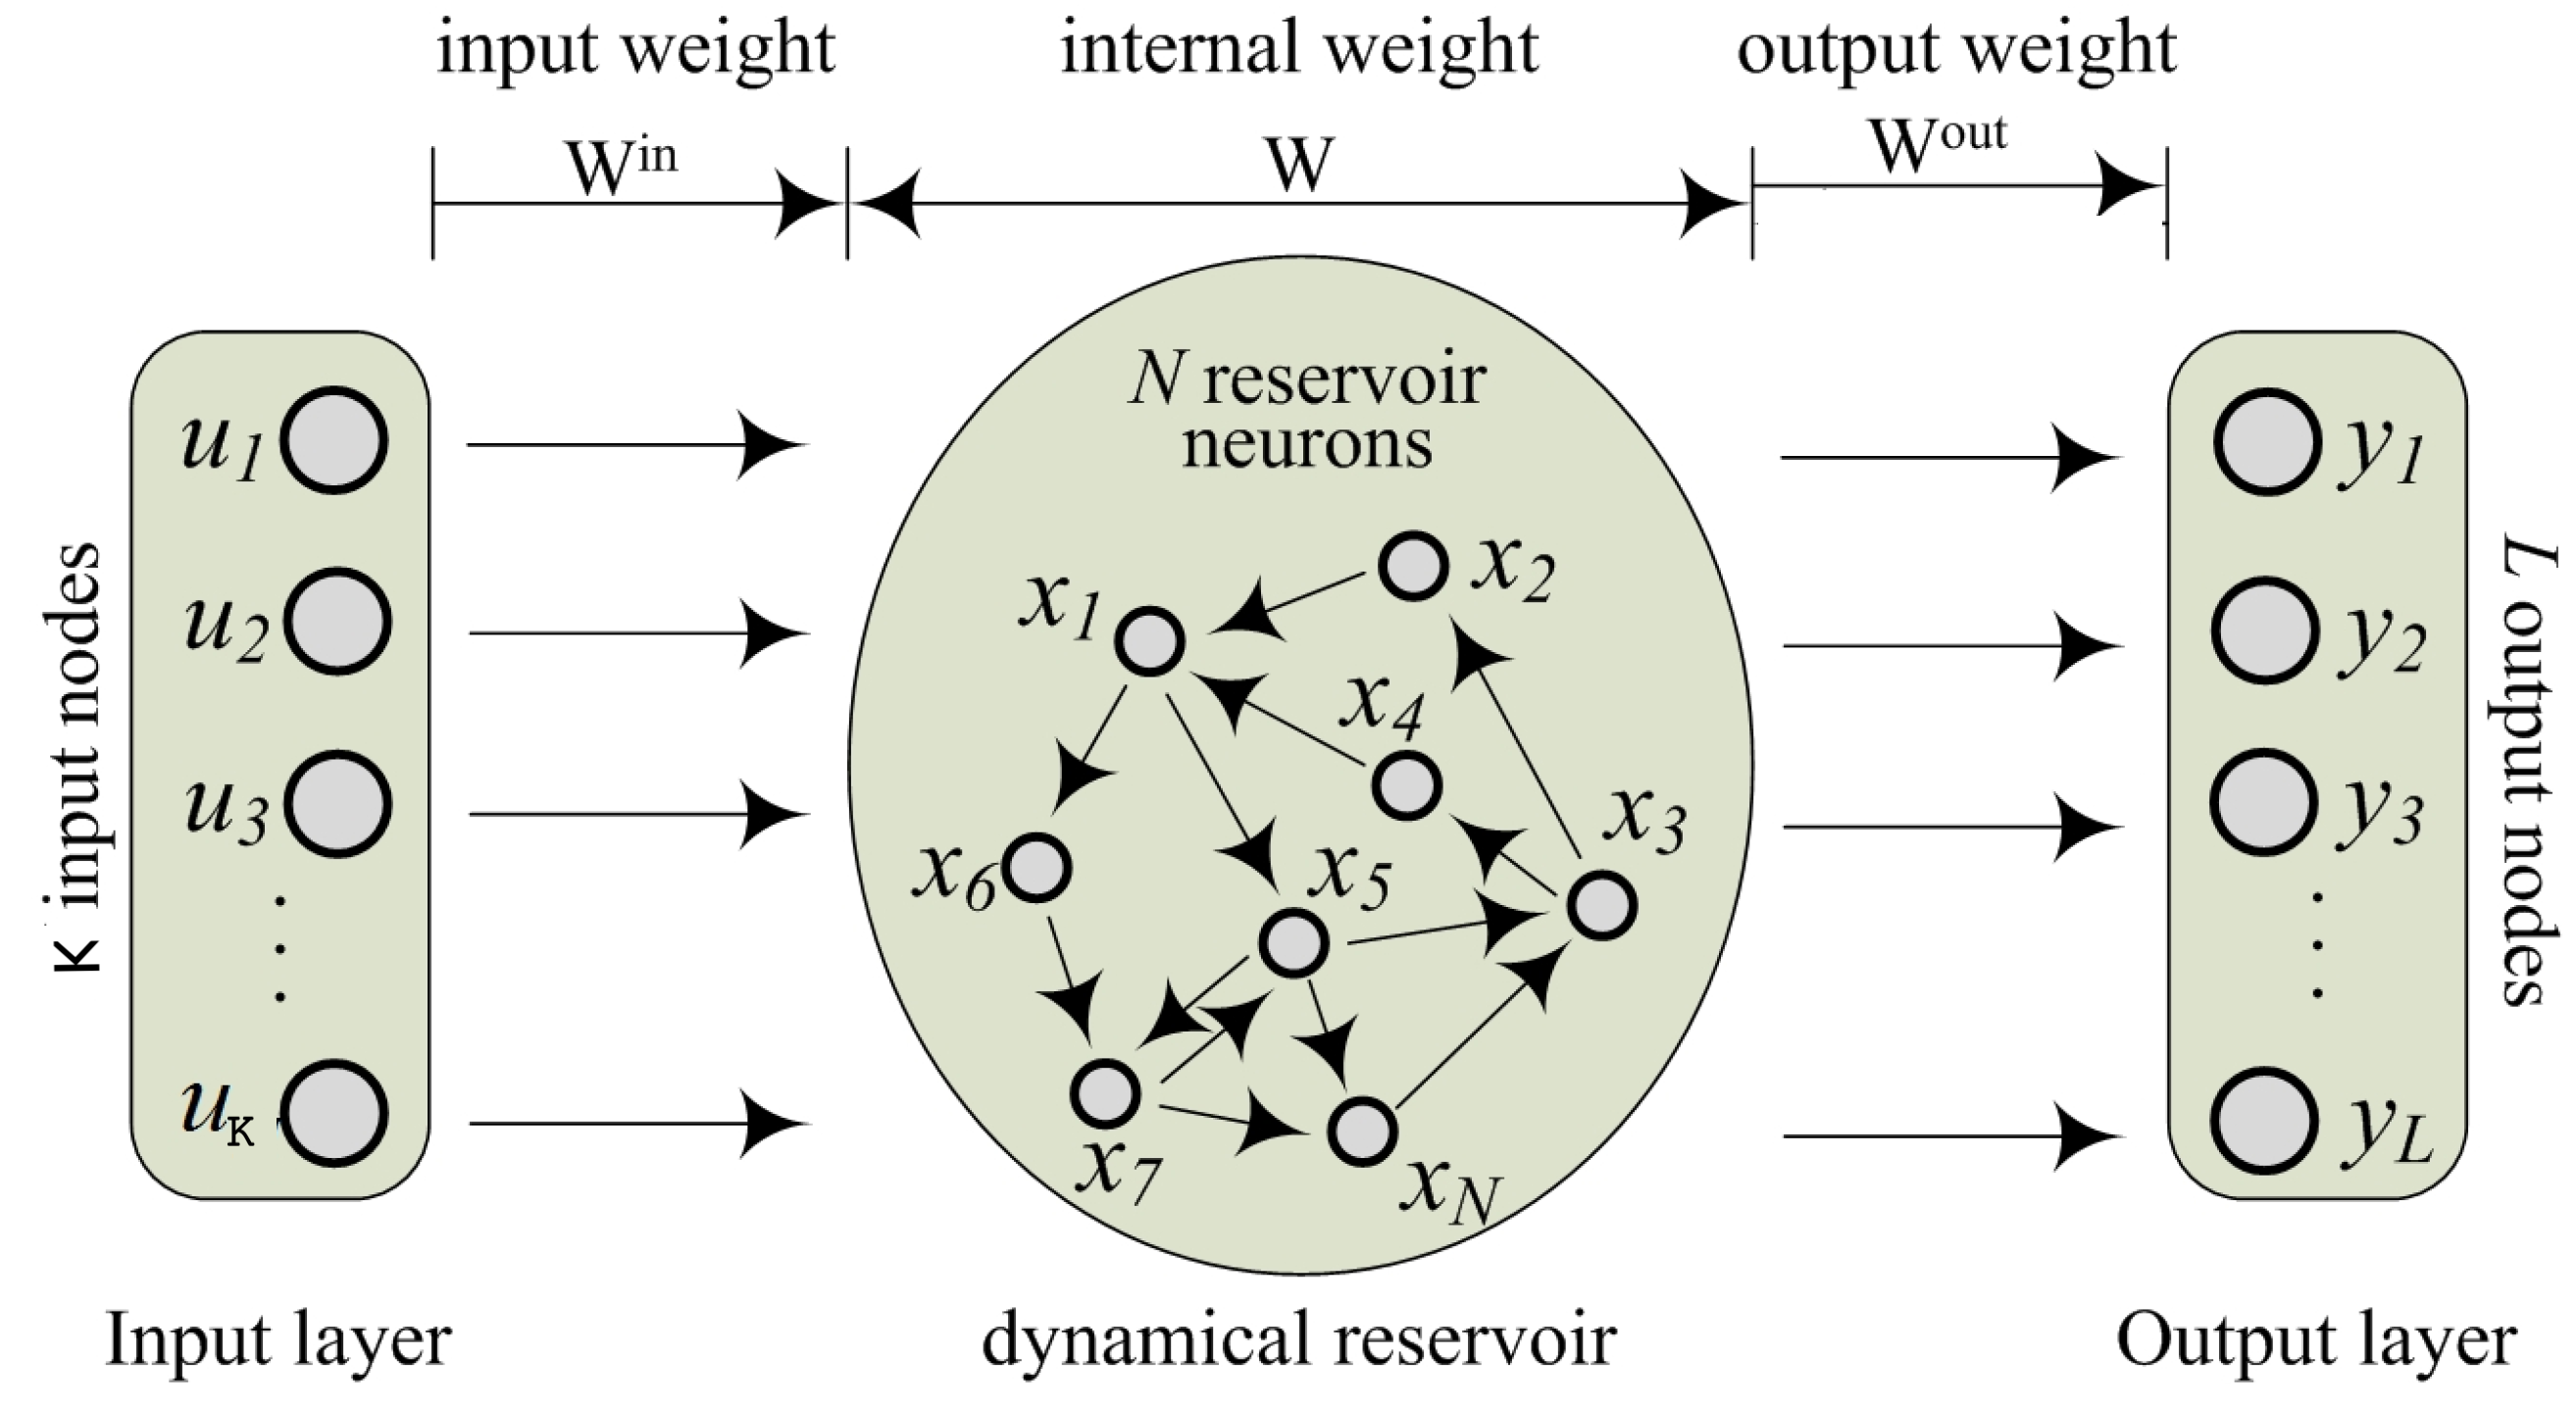
\includegraphics[width = 10cm]{./backgroundConcepts/images/esn1}
	 \caption{The basic schema of Echo State Network. Image source\cite{Li_2015}.}
  \end{figure}
 
  \subsection{Formalism}
  \subsubsection{Formulation of problem}
    Let a \textit{problem} or a \textit{task} in our context of machine learning be defined as a problem of learning  a task of prediction. Given a time series ${s(t)} = (s(t-M\Gamma),  s(t-(M-1)\Gamma), \hdots, s(t))$, our goal is  to predict the next few data points of the time series, $y = ( s(t + M\Gamma), s(t+(M+1)\Gamma),\hdots)$ such that $E(\mathbf{y}, \mathbf{y}^{target})$ is minimized where $y^{target}$ is the predicted values and  $E$ is the training error measure, for example, normalized root-mean-square error (NRMSE) \eqref{eq:nrmse}.
    \\
    
    % such that  the predicted values $y^{target}$ is close to the the real values of the corresponding data points in the time series $s(t)$ . Our goal is to minimize the the training error $E(y, y^{target}$), for example, normalized root mean square error(NRMSE). \\
    % \\a given input  $\mathbf{u}(n)\in \mathbb{R}^{Nu}$ and a desired output $\mathbf{y}^{\text{target}}(n) \in \mathbb{R}^{Ny}$. Our goal is to learn a function $\mathbf{y}(n) = y(\mathbf{u}(n))$ such that $E(\mathbf{y}, \mathbf{y}^{target})$ is minimized where $E$ is the training error measure, for example, normalized root-mean-square error (NRMSE) \eqref{eq:nrmse} \cite{reservoirComputing}.
    
	\subsubsection{Theory}
  We consider discrete time neural networks with $K$ input units, $N$ internal network units and $L$ output units. Each of these units at time step n has activation. Activations of input units at time step $n$ are $\mathbf{u}(n) = (u_1(n),\hdots,u_K(n))^{'}$, of internal units are $\mathbf{x}(n) =( x_1(n),\hdots,x_N(n) )^{'}$ and of output units are $\mathbf{y}(n) = (y_1(n),\hdots,y_L(n))^{'}$. Real valued connection weights for the input links are collected in the matrix $\mathbf{W}^{in} \in \mathbb{R}^{N \times K }$, for the synaptic links between the neurons within the network are collected in matrix $\mathbf{W} \in \mathbb{R}^{N \times N }$, and for the output weights are collected in matrix $\mathbf{W}^{out} \in \mathbb{R}^{L \times (K+N) }$ \cite{EchoStatesTechRep}. The connections from input to output are used and the corresponding connection weights are stored in matrix $\mathbf{W}^{out}$. The output units may optionally project back to internal units with connections. However,1 they have not been used in this experiment. A zero weight value can be interpreted as "no connection" \cite{Jaeger_TrainingRNNsTutorial.2005}. \\
  \indent \indent
  The activation of internal units are updated according to the discrete time state update Equation \eqref{eq:stateUpdate}.
   %
%   \begin{equation} \label{eq:stateUpdate}
%     \mathbf{x}(n+1) = f(\mathbf{Wx}(n) +  \mathbf{W}^{in}\mathbf{u}(n+1) + \mathbf{B} )
%   \end{equation}
   \begin{equation} \label{eq:stateUpdate}
    \mathbf{x}(n+1) = (1-\alpha)\mathbf{x}(n) + \alpha ( f(\mathbf{Wx}(n) +  \mathbf{W}^{in}\mathbf{u}(n+1) + \mathbf{B} ) )
  \end{equation}
   where $\mathbf{u}(n)$ is the externally given input, $f()$ denotes the component-wise application of unit output function ($tanh$ used for this experiment), $\mathbf{B} \in \mathbb{R}^N$ is the bias vector, and $\alpha \in \mathbb{R}^{N\times1}$ is a leaking rate.
   
   In ordinary ESNs, the current state $\mathbf{x}(n+1)$ of the network functionally depends only on the previous state $\mathbf{x}(n)$. This property is excellent for learning discrete chaotic signals with strong oscillations but imposes difficulties when dealing with continuous slow signals. To overcome this problem, we use networks with continuous dynamics.  Networks with continuous dynamics can be approximated by updating the network with a leaky integrator. The leaking rate $\alpha$ can be intuitively seen as the value that regulates  the amount of information preserved from the previous state and amount of information updated by the network update function. 
   With the value of $\alpha$ close to 0 the network state is changed very slowly as only a small ‘fraction‘ of the state is updated. On the other hand, when the values of $\alpha$ is closer to 1, the network state is updated very quickly. The leaking rate allows Echo State Networks to remember previous states across multiple update cycles allowing the network to learn continuous signals with long periods \cite{EchoStatesTechRep,erodriguez}.

% The leaking rate $\alpha \in \mathbb{R}^{N\times 1}$ of the reservoir nodes can be regarded as the speed of the reservoir update dynamics discretized in time.
%  The state update  Eq. \eqref{eq:stateUpdate} is modified to Eq. \eqref{eq:stateUpdateWithLeaky}. The values


%   \begin{equation} \label{eq:stateUpdateWithLeaky}
%     \mathbf{x}(n+1) = (1-\alpha)\mathbf{x}(n) + \alpha ( f(\mathbf{Wx}(n) +  \mathbf{W}^{in}\mathbf{u}(n+1) + \mathbf{B} ) )
%   \end{equation}
 
Each component of $\alpha \in \mathbb{R}^{N\times 1}$ can be optimized for the better performance of the network. However, this increases the number of parameters that need to be optimized. Therefore, to make the tuning process easier, the one dimensional vector is divided into three regions so that it has three different leaking rates or scaling factors. The entire vector $\alpha$ consists of three scaling factors which are the parameters that need to be optimized.
   
%     $\mathbf{x}(n)$ is $N$
%   dimensional state of the network at time point $n$, $\mathbf{W}$ is $N\times N$ matrix
%   consisting the weights of synaptic links connecting the neurons in reservoir, \textbf{W}$^{in}$ is $N\times K$ matrix consisting
%   weights of input links, \textbf{y}(n) is the output signal at time point $n$ and \textbf{B} is the bias vector of dimension $N$.

%  For our implementation, we have ignored output feedback to the network so the
%  state equation reduces to
%   \begin{equation} \label{eq:stateUpdate}
%   \textbf{x}(n+1) = f(\textbf{Wx}(n) +  \textbf{W}^{in}\textbf{u(n+1)} + \mathbf{B} )
%  \end{equation}

 The extended system state $\mathbf{z}(n) = [\mathbf{x}(n) ; \mathbf{u}(n)]$ is obtained 
 by the concatenation of system states and input signal at time $\mathbf{n}$. For each time point, $i = 1,\hdots ,n_{max}$, the extended system state is stacked row-wise in a state collection matrix $\mathbf{S}$. This process is known as harvesting reservoir state. The output is 
 obtained from the extended system states using Equation \eqref{eq:prediction}.
 \begin{equation} \label{eq:prediction}
   \mathbf{y}(n) = \mathbf{g}(\mathbf{W}^{out} \mathbf{z}(n) )
 \end{equation}
   % where $\mathbf{W}^{out}$ is $L\times(K+N)$ dimensional matrix of output
%    weights and
   where $\mathbf{g} = (g_1, \hdots,g_L)$ is unit output activation function (in our case identity) \cite{Jaeger:2007}.
  
   The $\mathbf{W}^{out}$ matrix consisting the weights of links connecting reservoirs to output nodes is obtained by the linear 
   regression of weights of desired outputs $\mathbf{d}(n)$ on the harvested 
   extended systems states $\mathbf{z}(n)$. $\mathbf{W}^{out}$ can be computed 
   efficiently by linear regression of $\mathbf{S}$ and $\mathbf{D}$ as given by Equation \eqref{eq:wout}.
   \begin{equation}\label{eq:wout}
 	\mathbf{W}^{out} =
      (\mathbf{S^{'}S} + \beta \mathbf{I})^{-1}\mathbf{S^{'}D}
 	 % \label{eq:linreg}
      \end{equation}
     
      where $\beta$ is the regularization coefficient $\mathbf{D}$ is 
      desired output vector\cite{Jaeger:2007}.
      
      
% \subsubsection{Leaky Integration}
% In ordinary ESNs, the current state $\mathbf{x}(n+1)$ of the network functionally depends only on the previous state $\mathbf{x}(n)$. This property is excellent for learning discrete chaotic signals with strong oscillations but imposes difficulties when dealing with continuous slow signals. To overcome this problem, we use networks with continuous dynamics.  Networks with continuous dynamics can be approximated by updating the network with a leaky integrator. The leaking rate $\alpha$ can be intuitively seen as the value that regulates how much information about the previous state is preserved and how much information is updated by the network update function. When $\alpha$ with its value close to 0 the network state is changed very slowly since only a small ‘fraction‘ of the state is updated. On the other hand, when $\alpha$ with its value close to 1, the network state is updated very quickly. The leaking rate allows Echo State Networks to remember previous states across multiple update cycles allowing the network to learn continuous signals with long periods \cite{EchoStatesTechRep,erodriguez}.

% % The leaking rate $\alpha \in \mathbb{R}^{N\times 1}$ of the reservoir nodes can be regarded as the speed of the reservoir update dynamics discretized in time.
%  The state update  Eq. \eqref{eq:stateUpdate} is modified to Eq. \eqref{eq:stateUpdateWithLeaky}. The values


%   \begin{equation} \label{eq:stateUpdateWithLeaky}
%     \mathbf{x}(n+1) = (1-\alpha)\mathbf{x}(n) + \alpha ( f(\mathbf{Wx}(n) +  \mathbf{W}^{in}\mathbf{u}(n+1) + \mathbf{B} ) )
%   \end{equation}
 
% Each component of $\alpha \in \mathbb{R}^{N\times 1}$ can be optimized for the better performance of the network, however, this increases the number of parameters that need to be optimized, with the increase in the size of Network. Therefore to make the tuning process easier the one dimensional vector is divided into three regions so that it has three different leaking rates or scaling factors. The entire vector $\alpha$ consists and the three scaling factor are the parameters that need to be optimized.